% Author: David L Patrzeba
% Team 1 Software Engineering

\documentclass[11pt,letterpaper,oneside]{memoir}
\usepackage{smiflstyle}
\usepackage{indentfirst}
\usepackage{float}

% Include Title page
\title{
{\color{color2} \hrule}\vspace{1cm}
\Huge{\color{color1} Project Proposal:\\The Paramount Investments League
\vspace{1cm}
{\color{color2} \hrule}\vspace{1cm}}
\Large{ \color{color2} Report 1\\
Software Engineering\\
14:332:452}
}

% define custom author layout (highly temperamental)
\author{\huge{\color{color0}Team 1:\\}\vskip.1in
\Large{\href{mailto:david.patrzeba@gmail.com}{David Patrzeba}\\
\href{mailto:eric.jacob.10@gmail.com}{Eric Jacob}\\
\href{mailto:evanarbeitman@gmail.edu}{Evan Arbeitman}\\
\href{mailto:christopher.a.mancuso@gmail.com}{Christopher Mancuso}\\
\href{mailto:dkarivalis@gmail.edu}{David Karivalis}\\
\href{mailto:jdlziegler@gmail.com}{Jesse Ziegler}}}

\date{\today}


\begin{document}
\titleGM    % use this instead instead of \maketitle

% Include Contributions page
{

Hyperlinks:\\
\begin{center}
\href{http://192.241.248.91}{Webapp Link}\\
\href{https://github.com/dkarivalis/SEP_SMIFL}{Project Repository}\\
\href{https://github.com/dkarivalis/SEP_SMIFL_reports}{Reports Repository}\\
\end{center}

Revision History:
\begin{longtable}{|p{1.6in}|p{2.6in}|}
\hline
{\large\color{color1}Version No.}&{\large \color{color1}Date of Revision}\\\hline
v.1.1&2/7/2014  \\ \hline
v.1.2&2/16/2014 \\ \hline
v.1.3&2/23/2014 \\ \hline
\end{longtable}

\vspace{20mm}\

}




\tableofcontents % create TOC
\pagebreak

% Chapter 1
% Include Customer Statement of Requirements
\chapter{Customer Statement of Requirements}

\section{Problem Statement}

The stock market, more specifically the New York Stock
Exchange(NYSE) and the Nasdaq play a pivotal role in the American
economy today. Both are signals of the strength of the private
sector and consumer confidence. It is thus no surprise that
more and more people want to be involved in these markets
and attempt to increase their own wealth.\\

There is however a barrier to entry for many people, both
young and old in participating.  That is why with Paramount
Investments League we are interested in a platform for interacting
with these markets and providing educational interfaces for
breaking down these barriers.  Users should be able to easily
register with the system and begin participating immediately.
They should be given an imaginary cash portfolio where they can
perform basic market orders such as buy and sell. These orders to
should mimic real market orders as closely as possible and should
include a brokers fee. More sophisticated market maneuvers should be
unlocked as the user progresses through an achievements ladder.\\

Paramount Investments League is geared towards a wide array
of audiences and expects a variety of users with varying knowledge
levels to participate. In order to maintain appeal amongst these
users the platform should provide rewards to users for acheiving
particular goals.  We would like to replicate the idea of
achievements or trophies similar to the Microsoft xBox and Sony
Playstation family of systems. These achievements can award users
with new abilities or additional cash to their portfolio as they rise
up the achievements ladder. Users should also be able to create leagues
to help further enhance the competitiveness of the game.\\

Leagues exist to allow multiple users to compete against a subset
of the global user base with individual league rules.  This allows leagues
to set particular goals in order to be declared the winner.  Leagues
will require a cash buy-in that will be pooled together and distributed
to the winner(s) as seen fit by the league creator. To help facilitate
these leagues, a leader board will be created for each individual league
such that users can see their progress. In addition to league leader boards,
mutliple global leaderboards will be available providing specific metrics
of comparison.\\

To help facilitate a better understanding of markets, market metrics
should be available to the user through news feeds of companies in
their portfolio, interactive charts, and a live ticker of current
trades happening on our platform. Users should be able to have granular
control of email and social media updates.\\

The entire experience should be unified across mobile, tablet, and the
desktop and combined with the above features provide an enthralling
core experience for users to learn about the stock market.\\


% Input Glossary
\section{Glossary of Terms}



\textbf{Achievement} -- Any set goal reached by an investor.
Achievement rewards can be managed by a league manager and
may include badges, capital, equity, etc.\\

\textbf{Transaction Ticker} -- Constantly updating scroll of
most recent trades across the market. Users can observe market
trends from global equities which may or may not already be
in their portfolio.\\

\textbf{Leaderboard} -- Global or league based ranking system
determined by overall net worth of player.\\

\textbf{Security} -- A tradable asset of any kind. Can include
debts, equities, or derivatives. For the purpose of this game,
we will be dealing primarily with equities.\newline

\textbf{Dividend} -- A payment made by a corporation to its
shareholders, generally as a distribution of profit. It is
usually distributed as a fixed percent of shareholder value.\\

\textbf{Derivative} -- Any financial contract which derives its
value from another asset or index.\\

\textbf{Option} -- Gives the user the option to buy or sell an
asset at a specified price on or before a given date. The buyer
and seller are both obligated to fulfill the transaction on the
given date if the option is taken.\\

\textbf{Future} - Allows the buyer to buy an asset at its current
price and pay for it at that price in the future. A future is
generally exchange traded. The buyer and seller are both obligated
to fulfill the transaction on the given date if the future is taken.\\

\textbf{Forward} -- Allows the buyer to buy an asset at its current
price and pay for it at that price in the future. A forward is a
private agreement between buyer and seller not necessarily based around
market equity. The buyer and seller are both obligated to fulfill
the transaction on the given date if the future is taken.\\

\textbf{League} -- A market simulation with a pre-determined rule set
and several investors with a common goal to determine a winner. Goals
can vary across leagues as determined by league managers. Investors can
choose to opt into a private league, public league, or no league at all.\\

\textbf{Portfolio} -- A detailed account of assets associated with a
particular investor in a given league. Portfolios are unique to each user
and will contain specific details such as earnings, losses, performance,
averages, as well as detailed asset performances of equities within the
given portfolio.\\

\textbf{League manager} -- The league manager will have the responsibility
of added and/or removing investors from the league. League managers
control settings, and victory conditions for a particular league. League
managers maintain their manager status only for the league in which they
have created.\\

\textbf{Order} -- An investor must place an order for the purchase or
sale of an asset.\\

\textbf{Stock} -- A type of asset that represents equity in a company.
\begin{itemize}
    \item \textbf{Ask Price} -- The price at which a trader is willing
                                to sell a stock.
    \item \textbf{Bid Price} -- The price a trader is willing to pay for
                                a stock.
    \item \textbf{Bid-Ask Spread} -- The bid-ask spread describes the
                                     difference in price between the bid
                                     and the ask. These two prices are
                                     marginally different, but always with
                                     the ask being the more expensive of the
                                     two. It represents the friction inherent
                                     in trading a stock.
\end{itemize}

\textbf{Ticker Symbol} -- an abbreviation used to uniquely identify publicly
traded shares of a particular stock on a particular stock market.\\

\textbf{Symbol List} -- a list of a market/several market's ticker symbols.\\




% Chapter 2
% Include System Enumerated Requirements
\chapter{System Requirements}

\section{User Stories}

\renewcommand\arraystretch{2}
\begin{longtable}{|p{0.6in}|p{4.6in}|p{0.5in}|}
\hline
{\large \color{color1}Identifier}&{\large \color{color1}User Story}&{\large
  \color{color1}Weight} \\ \hline
ST-1&As a user, I can create an account without registering with the website
in order to participate in Paramount Investment League.&10 pts \\ \hline

ST-2&As a user, I can access the application across multiple platform paradigms
so that I may continue to participate when I don't have access to a desktop
computer.&10 pts \\ \hline

ST-3&As a user, I can join or create leagues with self-selected goals so that I
may compete with others in a simulated stock market environment based on
near real-time stock data.&10 pts \\ \hline

ST-4&As a user, I can search for companies by stock symbol and be presented with
their current financial information so that I may research future investments.&6
pts  \\ \hline

ST-5&As a user, I can browse a companies profile and view the performance data
over a configurable span of time so that I may determine whether or not I want
to invest in them.&6 pts  \\ \hline

ST-6&As a user, I can buy or sell stocks so I may build my portfolio.&10 pts
\\ \hline

ST-7&As a user, I can earn badges(achievements) that reward me with additional
capital or new features for accomplishing predefined tasks.&10 pts \\ \hline

ST-8&As a user, I can manage my portfolio within a league to track my
investments.&8 pts  \\ \hline

ST-9&As a user, I can visually track my finances via graphs and charts so I may
more easily manage my portfolio.&4 pts  \\ \hline

ST-10&As a user new to the stock market, I will have access to an educational
interface that teaches me about the stock market via pop-up dialogues.&6 pts
\\ \hline

ST-11&As a user, I can see trades being made by all other users in real-time via
a stock-ticker like marquee so I may have a quick overview of current trends.&3
pts  \\ \hline

ST-12&As a user, I can see the performance of other users' portfolios so I may
observe the investment habits of others.&2 pts  \\ \hline

ST-13&As a user, I can view a portfolio leader board so I may have a summary of
relative performance between users in my league.&1 pt   \\ \hline

ST-14&As a user, I can opt to receive periodic e-mail notifications of my stock
performance or trades so I may be kept up to date even when not actively viewing
the site.&3 pts  \\ \hline

ST-15&As a user, I can additionally link my account with social media sites so
I may share my fantasy league experience with friends.&1 pt   \\ \hline

ST-16&As a league manager, I can add league rules, a league name, and a league
logo to personalize my league.&8 pts  \\ \hline

ST-17&As a league manager, I may invit I want to join,and assign.&8 pts
\\ \hline

ST-18&As a league manager, I can create league announcements.&4 pts  \\ \hline

ST-19&As a site administrator, I can view reports of and delete leagues that are
inactive.&2 pts  \\ \hline

ST-20&As a site administrator, I may post front page news or announcements.&3
pts  \\ \hline

ST-21&As a site administrator, I may have access to a user count, number of
active leagues, total leagues, quantity of daily transactions, the most/least
popular stocks, and newly created so I may have reliable site statistics. &9 pts
\\ \hline

\end{longtable}



% Include FURPS
\section{Nonfunctional Requirements}



\subsection{Functionality}
Additional features for security will be enabled through the use of a
OpenID and OAuth through a third-party library. There exists several packages
for the purpose of authentication and authorization of users. Key authentication
features are the ability to encrypt and store passwords, provide recovery
options for users that have forgotten their password, and store a cookie to
validate the session.


\subsection{Usability}
A key point in the design of this application is ease of use and appeal to the
users. The application should be interactive, informative and consistent across
multiple platform paradigms. Additionally the application will be used to
provide the educational interfaces noted in ST-9 which should be able to be
toggled on and off so that users can always view the information again.


\subsection{Reliability}
In order to ensure that there is no confusion to the user in the case of the
internet or server failure, all transactions end with a final confirmation, and
no changes to the account are made until after this confirmation. The user's
portfolio will thus always be in a consistent state and will be restored when
the user is able to log back in. A user that leaves the application and returns
later will still be logged in. Server failure should also be dealt with by
keeping backups of user data.  Proper care should also be taken to handle a
situation where a particular stock source is not available (i.e. Yahoo Finance).


\subsection{Performance}
In order to have a great performance, the website should be as lightweight as
possible by keeping hardware demands to a minimum on both the client and server
sides. For it to be efficient, any task initiated by the user should be
completed in a timely manner. The web server should be able to serve concurrent
requests especially when a large number of users are logged in. Any frameworks
used should be lightweight but consideration should be taken not to prematurely
optimize.


\subsection{Supportability}
It should be feasible to extend pr update any server components and include
improved versions of modules which can be installed only by administrators. For
scaling purposes, it should be made easy to include an additional number of
servers to achieve load balancing. The system should be platform independent so
that it is easy to move to newer technologies or the next versions of web
server. The system itself should also be backed up to a remote server for the
sole purpose of extending functionality and testing new features in a
controlled environment.



% Input On Screen Appearance Requirements
\section{On-Screen Appearance Requirements}



There are a few on screen requirements that will be universal to the entire site:\\
\renewcommand\arraystretch{2}
\begin{longtable}{|p{0.6in}|p{4.6in}|}
\hline
{\large \color{color1}Identifier}&{\large \color{color1}Requirement} \\ \hline

OSR-1& Every page has a scrolling ticker across the bottom of the page to update the user
on stock movement. \\ \hline

OSR-2& Every page, with the exception of the login page, will have
navigational links across the top, the user's username and their current position in
the leaderboard. \\ \hline

\end{longtable}


There are also the following requirements for specific pages:\\

\renewcommand\arraystretch{2}
\begin{longtable}{|p{0.6in}|p{4.6in}|}
\hline
{\large \color{color1}Identifier}&{\large \color{color1}Requirement} \\ \hline

OSR-3&  A custom 404 not found page will be displayed to a user when they try to  access
a URL/URI that doesn't exist or is not designed for them to be accessing. \\ \hline

OSR-4& On the portfolio page users will find currently owned stocks, charts and graphs,
trade transcations, and a news feed. \\ \hline

OSR-5&  The leaderboard view will contain users ranked by the top networth from their
respective portfolios. \\ \hline

OSR-6&  The login page will present the user with login icons representing the service
they can use to log into our system, eg: google+, facebook, etc. \\ \hline

\end{longtable}


\begin{figure}[H]
\centering
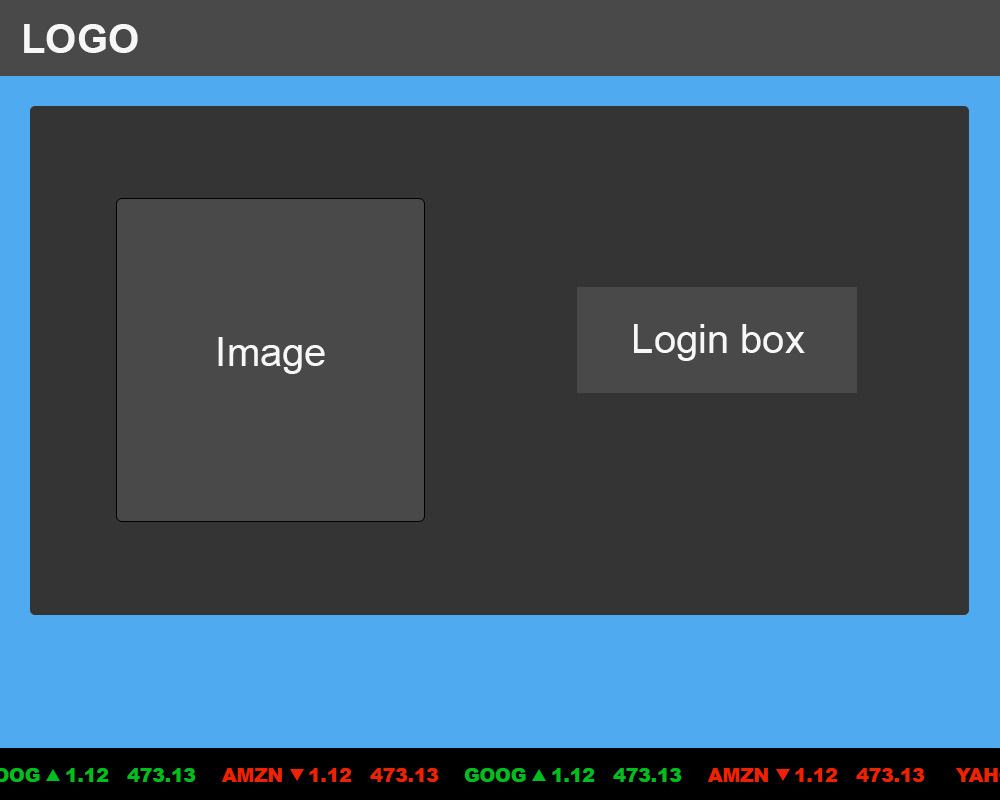
\includegraphics[width=5.5in]{./img/mock/loginmock.jpg}
\caption{Basic on screen requirements of login page}
\label{ui:mockup}
\end{figure}


% Chapter 3
% Include Functional Requirements Spec
\include{./tex/functionalrequirements}

% Chapter 4
% Include UI Specification
\chapter{User Interface Specification}
\label{uispec}
% This section contains mockups, descriptions,
% and explanations, lots of graphics
\section{Preliminary Design}

The user interface (UI) for Paramount Invesments Leagues will act as a command center
for users to interact with their portfolio, leagues they are a part of, and conduct
research on potential orders. More specifically, the command center will act as the
primary; but not the only; view for users to interact with the system.  The command
center will provide a snapshot of the users current portfolio and its value, their
global rank, a dash to perform market orders, a news feed, and a graphing dash in order
to quick analysis of stock performance.  The UI will persist a users global rank across
all views as well as a ticker of current trades being placed through the Paramount
Investment League.\\

The UI should be lightweight so as not to burden our more restrictive target platforms
of mobile and tablet.  The colorscheme will be chosen to be easy on the viewer, though
this is subjective, the colorscheme will be a basic pallet of grey/black/white/blue,
tending toward pastel and web supported colors.\\

The UI will be built on top of Twitter's open source Bootstrap CSS\cite{wiki:boot}
framework to help
facilitate deleriving content to the three target platforms, desktop, mobile, and tablet.
Bootstrap provides a mobile first design philosophy, but can be customized to target
specific platforms.\\

\subsection{Landing Page and Login}

Paramount Invesment League is designed around allowing users to easily begin using the
service, also know as "zero effort" resgistration. In order to accomplish this, the
system does not require the user to register a new user name/account with our system,
but instead piggybacks on OpenID\cite{wiki:open} and OAuth\cite{wiki:oauth} allowing users to
use their Google,
Facebook, Twitter, and other OpenID/OAuth accounts to login. You'll also notice that
upon initial visit, the header is empty providing no navigation, this may be relaxed in
the future to allow the user to explore some of the features of the website that don't
require user authentication such as stock research. (\em See figure 3.1 \em)\\

\begin{figure}
\centering
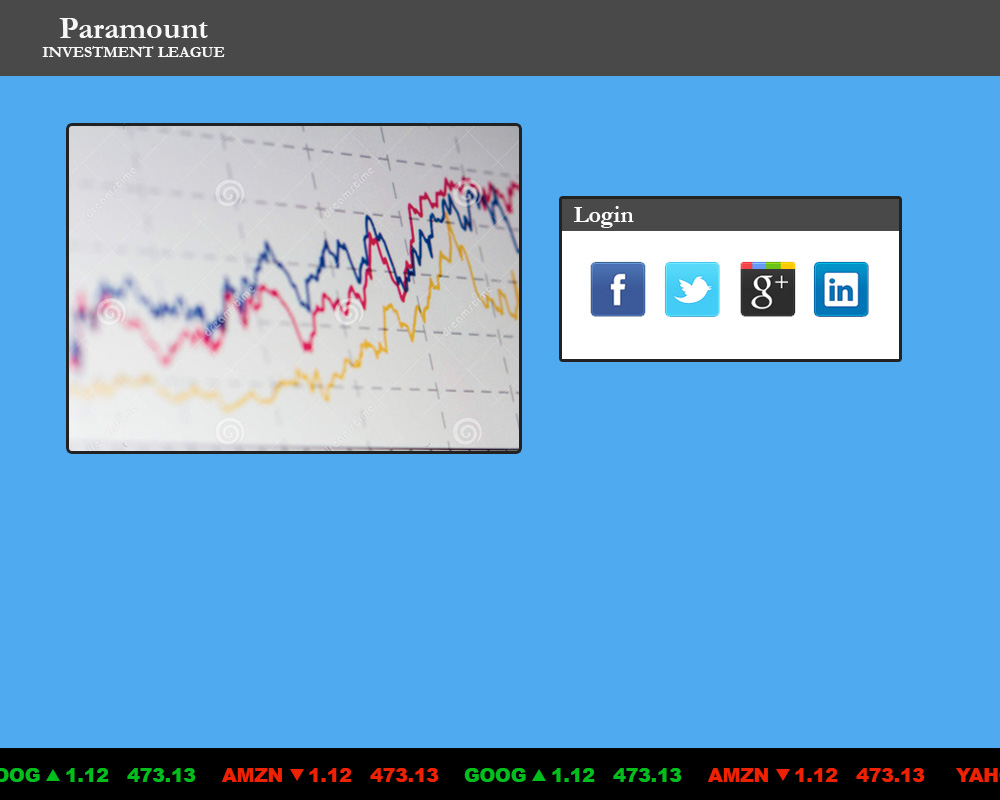
\includegraphics[width=5.5in]{./img/mock/login.jpg}
\caption{First iteration of Landing/Login page.}
\end{figure}

\subsection{Global Header}

The header (\em see Figure 3.2 \em)across the website will remain persistant across the
website once the user is logged into the system.  Navigation is done between essentially
4 views in the following order, My Portfolio, Stock, League, Leaderboard,.  These names
are placeholders and will most likely be My Portfolio, My Leauges, Leaderboards,
Analyze Assets. The 'My Leagues' and 'Leaderboards' will be turned into drop downs as
users expand into leagues to allow quick navigation.\\

The website name will also navigate to My Portfolio. The username will be replaced by the
users actual username, and below it will be the users global rank.  The rank will be
highlighted in red or green depending on whether they have improved their position on the
day, or it has declined.  It will also indicate how many spots they have moved.\\

\begin{figure}
\centering
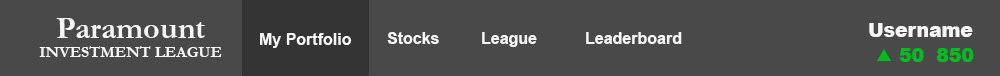
\includegraphics[width=5.5in]{./img/mock/topbar.jpg} %change with header
\caption{Preliminary design for a global header. This users is up 50 spots for the day.}
\end{figure}

\subsection{Global Ticker}

One interesting feature of Paramount Investment Leagues will be its active ticker at the
bottom of the website.  This ticker will be seen in all views, including the Landing Page
once there is enough volume to keep the ticker full.  The ticker serves two goals, one for
new users, and one for existing users.  The first goal is to entice new users to
participate by demonstrating that the app is being widely used. The second goal is to give
a snapshot to existing users of assets that are "on the move" so that they can attempt to
remain competetive. The ticker can be seen at the bottom of all the figures.\\

\subsection{My Portfolio}

The 'My Portfolio' (\em see Figure 3.3 \em) view of the  website will act as the command
center for a user wanting to get news about companies/assets in their portfolio, perform
an order, or conduct quick graphical anaylsis of assets in their portfolio and compare
them to any other asset available for trade through the platform.\\

More importantly, it provides a snapshot of the users portfolio including a scrollable list
of all the assets inside the portfolio and a summary of said assets.  In the future, assets
will be 'clickable' and will take the user to a summary page of that asset, but that is not
planned for the initial 2 iterations.\\

\begin{figure}
\centering
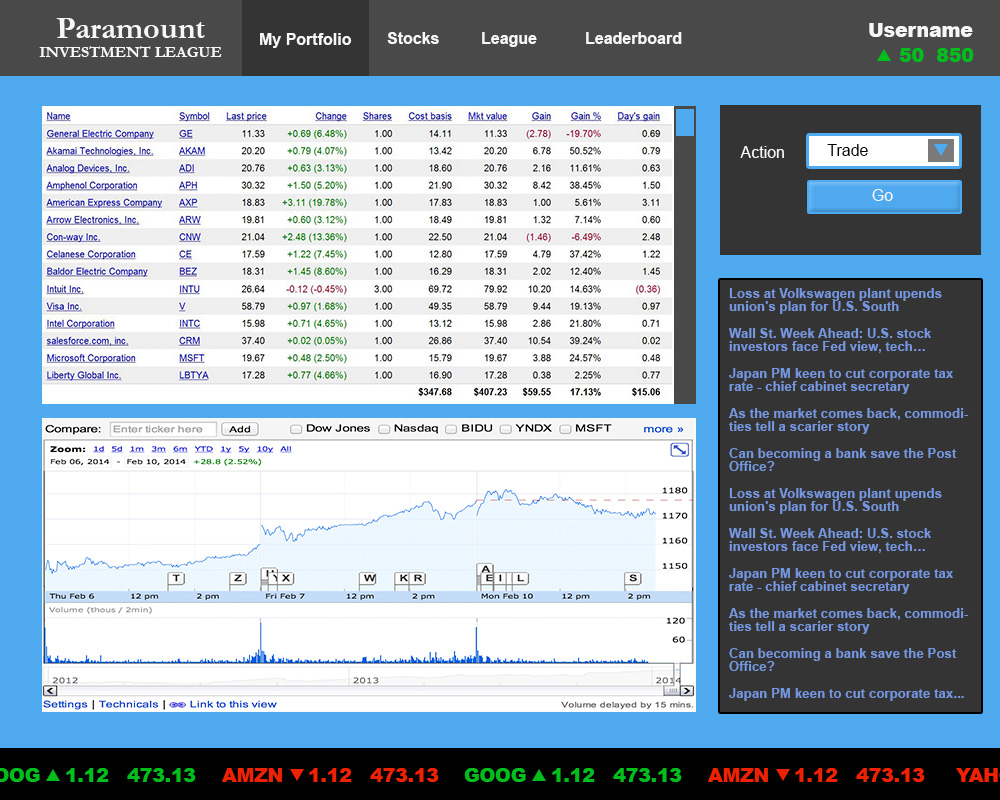
\includegraphics[width=5.5in]{./img/mock/portfolio.jpg}
\caption{The preliminary design of the 'My Portfolio' view.}
\end{figure}

\subsection{Leagues}

The 'League' (\em see Figure 3.4 \em) view will present a user that isn't a part of a league
the ability to create a new league of join an existing league.  Not shown in
\em Figure 3.4 \em is the view that a user who is a part of a league.  This view will still
persist the join/create dialogues, but will also present a list of all the leagues that user
is a part of, their rank within said league, and their movement within said league.\\

\begin{figure}
\centering
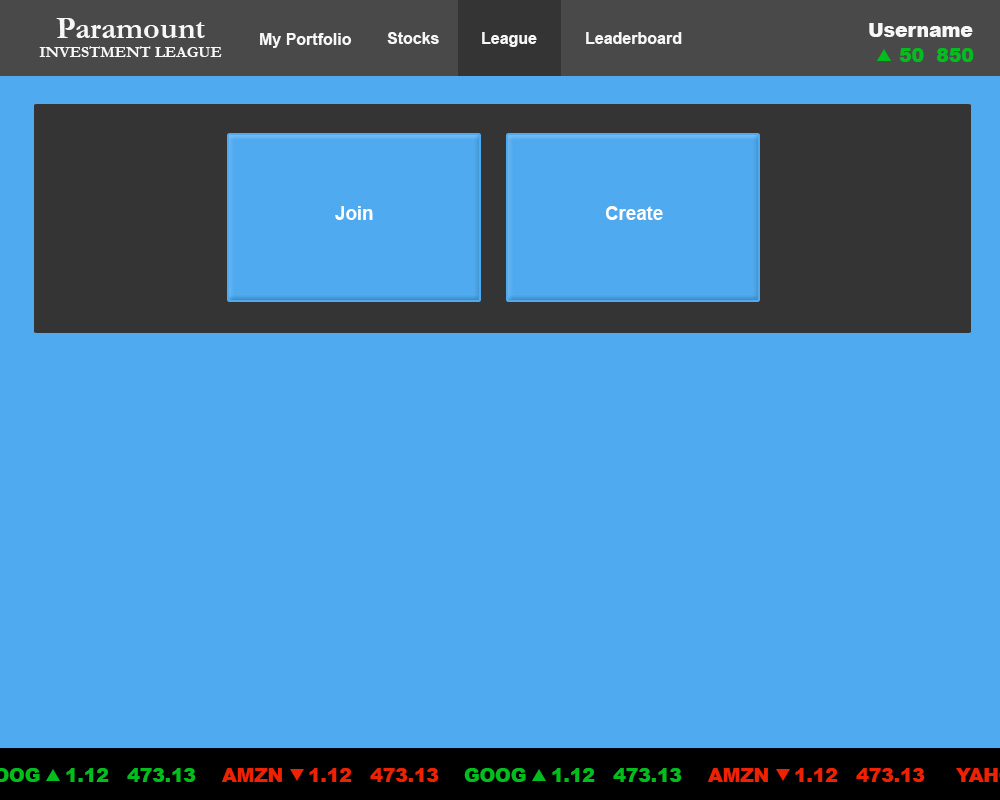
\includegraphics[width=5.5in]{./img/mock/league.jpg}
\caption{This is the league creation/join view. This would be the view presented to a user
that is a part of no league yet.}
\end{figure}


\subsection{Leaderboards}

The 'Leaderboards' (\em see Figure 3.5 \em) view will present the user with a partial view
of the full leaderboard for a given league, or for every user.  It will show their rank,
their movement, the value of their portfolio as well as the same stats for all other users
around them.  The view will be scrollable if there are more records then can be displayed,
and will center the user in the middle of the view unless they are at the top or bottom
of the board.\\

\begin{figure}
\centering
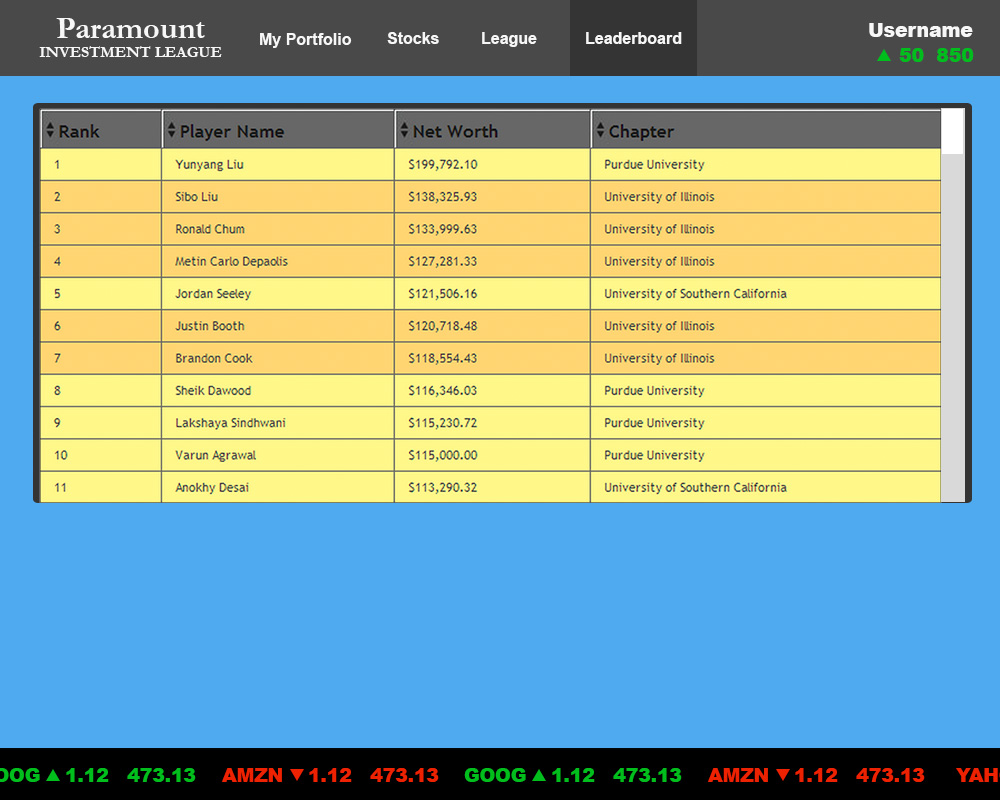
\includegraphics[width=5.5in]{./img/mock/leaderboard.jpg}
\caption{Here is the leaderboard view which will be the same for both leagues and global
leaderboards. This view represents a global leader board.  The colorscheme of this view
here is incomplete and will fall inline with the remainder of the site.}
\end{figure}

\subsection{Asset Analysis}
The 'Stocks' view (\em see Figure 3.5 \em) will be renamed to more align its function
with its name, which is to analyze assets. It will a more in depth way of anaylzing an
asset versus what is available in the 'My Portfolio' view.  There will be a news feed
at the bottom of assets that you are searching for. There will also be a more formal
analysis of asset data presented including P/E ratio, 52 week range, Volume, EPS, etc.
This isn't shown in the figure, but will one-half to two-thirds of the space that
has been set aside for the news feed.\\

This is also one of the views and functionalities that has been identified to not require
the user to be logged in.  While it will not be availble to non-users in the intial product,
it can be made available in future releases.\\

\begin{figure}
\centering
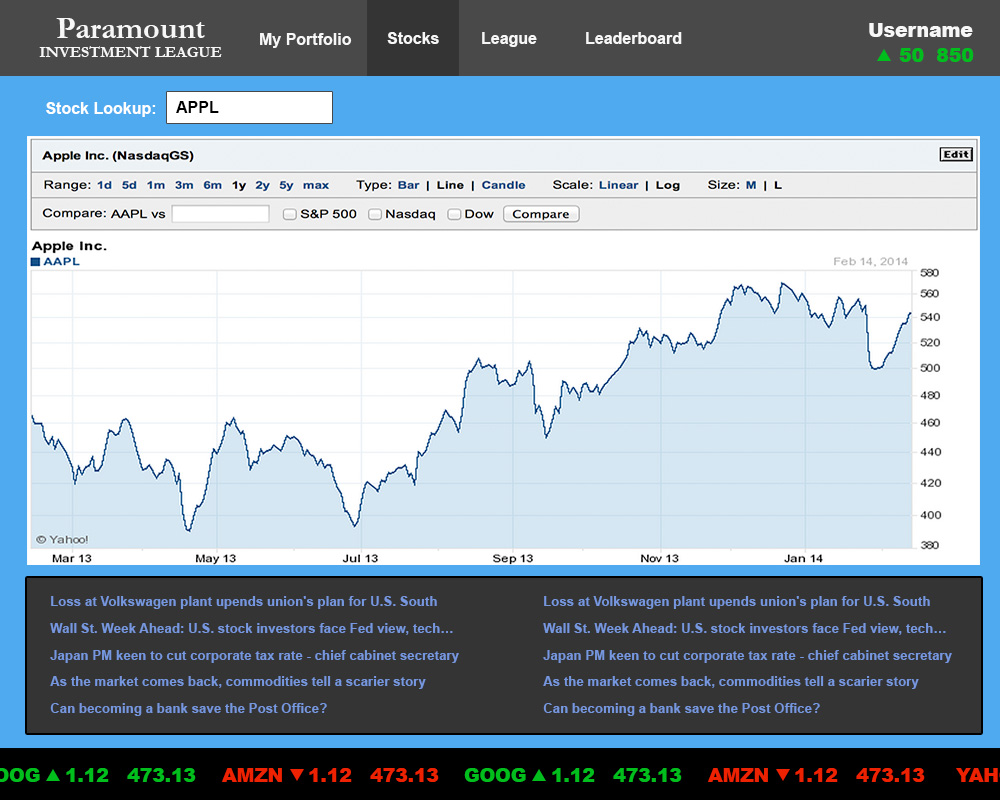
\includegraphics[width=5.5in]{./img/mock/stocks.jpg}
\caption{The preliminary view for asset anaylsis.}
\end{figure}


% This section contains lots of explanations
% of user effort and ease of access
% See Appendix A for examples to boost grade
\section{User Effort Estimation}

Several of the most common usage scenarios for Paramount Investment Leagues:\\

\begin{center}
\begin{tabular}{| l | l | l |}
\hline
\textbf{Usage Scenario} & \textbf{Clicks} & \textbf{Keystrokes} \\ \hline
Login \& Register & 2-3 & 0-1 \\ \hline
Place an Order & 4-6 & 2-12 \\ \hline
Join a League & 3-4 & 0-50 \\ \hline
Create a new League & 6-7 & 11-100 \\ \hline
Analyze Asset & 2 & 2-5 \\ \hline
View Leaderboard & 2 & 0 \\ \hline
\end{tabular}
\end{center}

\subsection{Login \& Register}

Assume the user has come to the domain and wishes to Login if already registered, or
register if already a user:\\
\begin{itemize}
\item \textbf{Navigation: }
\begin{enumerate}
\item Click on OpenID icon (Google, Facebook, Twitter, etc).
\item Click on your account (optional for multiaccounts).
\item Click on login, or hit enter.
\end{enumerate}
\end{itemize}

\subsection{Place an Order}

Assume the user has already logged in and they wish to place an order:\\

\begin{itemize}
\item \textbf{Navigation: }
\begin{enumerate}
\item Navigate to 'My Portfolio', 0-1 clicks.

\end{enumerate}
\item \textbf{Data Entry: }
\begin{enumerate}
\item Select order type from drop down, 2 clicks
\item Click textbox to enter asset name. 1 click
\item Enter assets name eg: 'G', 'O', 'O', 'G', 1-4 keystrokes
\item Press tab to specify number of shares, 1 keystroke (user could also execute 1 click)
\item Enter the number of shares, 1-7 keystrokes
\item Click execute, 1 click
\end{enumerate}
\end{itemize}

\subsection{Join a League}

Assume that the user wishes to join a league and is logged in:\\

\begin{itemize}
\item \textbf{Navigation: }
\begin{enumerate}
\item Click on League, 1 click
\item Click on Join, 1 click
\end{enumerate}
\item \textbf{Data Entry: }
\begin{enumerate}
\item Click on a League, or enter its name, 1 click or up to 50 keystrokes
\item Click on confirmation dialogue, 1 click
\end{enumerate}
\end{itemize}

\subsection{Create a League}

Assume that the user wishes to create a league and is logged in:\\

\begin{itemize}
\item \textbf{Navigation: }
\begin{enumerate}
\item Click on League, 1 click
\item Click on Create, 1 click
\end{enumerate}
\item \textbf{Data Entry: }
\begin{enumerate}
\item Enter its name, 1-50 keystrokes
\item Select ruleset from dropdown, 2 clicks
\item Fill in parameters, 1-2 clicks and 10-50 keystrokes
\item Click on confirmation dialogue, 1 click
\end{enumerate}
\end{itemize}

\subsection{Analyze an Asset}

Assume that the user is logged in and they want to start an in depth analysis of an asset:\\

\begin{itemize}
\item \textbf{Navigation: }
\begin{enumerate}
\item Click on Stock, 1 click
\end{enumerate}
\item \textbf{Data Entry: }
\begin{enumerate}
\item Click on the textbox for entering an asset name, 1 click
\item Enter an asset name, 1-4 keystrokes
\item Hit enter, 1 keystroke
\end{enumerate}
\end{itemize}


\subsection{View Leaderboard}

Assume that the user has logged in and wants to veiw a leaderboard:\\

\begin{itemize}
\item \textbf{Navigation: }
\begin{enumerate}
\item Click on Leaderboard, 1 click
\item Click on Select Legue/Global, 1 click
\end{enumerate}
\end{itemize}



% Chapter 5
% Domain Analysis
\chapter{Domain Model}

% Preface the high-level organization of the domain
\iffalse
At its highest level, Capital Games consists of a few subsystems
working together and coordinated by an internal controller. The
end user interacts with the application through either a web browser
or by directly submitting HTTP requests to the server. These actions
are equivalent because user actions are translated into RESTful actions
and interpreted equivalently by an appropriate RESTful controller. \cite{wiki:restful}
Once a controller is invoked, it consults the 
internal subsystems before responding to the request. Each of the 
subsystems can be identified by the purpose they serve in relation
to the application. 

% Concept Definitions
\section{Concept Definitions}

\subsection{Database}
By its nature as a data-driven site, data persistence
is core to Capital Games. Therefore, a database subsystem is necessary. 
A challenge often encountered when using databases in an application is
the translation of database-native datatypes to the more varied datatypes
employed by dynamic applications. \cite{wiki:orm} To simplify this,
Capital Games uses the ActiveRecord object-relational mapper to abstract
the logic between the database and the system as a whole. Only privileged portions
of the system have access to the database. This maintains the safety of the
data while also allowing it to be manipulated more precisely. Per the convention
of MVC-style application style architecture 
% insert reference here for later chapter
(upon which we base our application, described in more detail later), these 
are known as the Models. The database is explored in more detail in the Data Structures section.

\subsection{Finance API Adaptor}
The data for the application comes from a third party source, Yahoo! Inc. Yahoo!
provides both nearly-real-time and historical data on most U.S.-traded stocks.
Yahoo! exposes this data through a web API service in which a party can make
up to several thousand requests against Yahoo!'s databases daily. The party
simply enters arguments into an HTTP request which is interpreted by Yahoo!
as a database search, runs the query, and returns the results in CSV format. \cite{gummy}

In order to interact with the web service, we employ an adaptor plugin which
translates between the various syntaxes used by Yahoo! and our own system.
Any and all parts of the application which require access to a live data-stream
invoke the Finance Adaptor subsystem, which in turn queries Yahoo!. This
modularity enables multiple subsystems of the application to have access to live data
when necessary.

\subsection{Queueing (Asynchronous Task) System}

Fundamentally, Capital Games is about placing trading orders for various stocks. 
Though the simplest type, market orders, are executed almost immediately after being 
placed, stop and limit orders may not be executed for quite some time. \cite{inv:market}
\cite{inv:stop} \cite{inv:limit} This begs the question of how to perform a trade
at some undetermined time after the order is placed. 
Upon further inspection, a few other functions of the site depend on a similar capability.
In order to update the user portfolio database regularly or send out newsletters, the system 
must be able to asynchronously execute certain tasks. Enter a Queueing System.

Whenever a task needs to be performed asynchronously, the task is entered into a 
designated portion of a Redis database, configured as a queue. Background "workers" 
(processes) perform tasks as they arrive. Tasks can also be scheduled to occur at specific
times or intervals. In this way, everything from polling the datastream for stock updates
to performing scheduled updates and e-mails can be coordinated by a single system.

\subsection{Views Generator}

Finally, when all data have been collected and a response needs to be rendered, those data
are delivered to a subsystem which dynamically generates the content
which are served up to the end-user. The Views Generator contains various modules which
simplify translating the data to web-standard HTML and Javascript.

\subsection{Mailer System}

Capital Games is designed to periodically alert users as to their portfolio performance.
This is performed by the Queueing System in conjunction with the Mailer system.
The framework we employ natively contains a robust mailing system called Action Mailer,
which generates content dynamically at runtime. \cite{action:mailer} This allows us to perform calculations
on leagues and then include that into emails, in addition to raw data.

%\begin{itemize}
%\item \textbf{Users}: Every end-user of the application needs both a private and
%public facing identity on the site.
%
%\item \textbf{Site Administrators}: The site needs a few global administrators
%who can delete posts and ban users which are innappropriate, as well
%as perform several maintenance features.
%
%\item \textbf{Leagues}: Every end-user is participating in one or more leagues.
%
%\item \textbf{Investors}: Because an end-user can participate in multiple leagues,
%and each instance of the user can have a separate amount of money, margin,
%etc., it is necessary to maintain a separate identity for each of these 
%instances -- \emph{investors}.
%
%\item \textbf{League Manager}: Every League should have a superuser who is 
%able to invite other players, perform moderation, and change settings.
%\end{itemize}
%
%Although not actors themselves, from UC-4 (page \pageref{UC-4}) and UC-5 
%(page \pageref{UC-5}) it is apparent that end-users are implicitly 
%requesting and manipulating data for their orders and portfolios. These,
%too, become part of the application domain.
%
%\begin{itemize}
%\item \textbf{Orders}: When an \emph{Investor} places any type of order, it
%needs to be tracked. 
%\item \textbf{Stocks}: Whenever an Investor is tracking the performance of a
%stock, those data need to be stored locally. Stocks is a unified 
%data object to contain those data.
%\end{itemize}
%
%One of the actors at the back end of UC-3 (page \pageref{UC-3}) and UC-4
%(\pageref{UC-4}) was the Financial API, responsible for accessing the 
%market data stream. 
%
%\begin{itemize}
%\item \textbf{Financial API}: This module presents an interface for requesting market
%data, both live and historical. 
%\end{itemize}
%
%Upon further analysis, it becomes apparent that the domain model is missing
%functionality responsible for asynchronously executing jobs. This is another
%core feature of the site, without which Stop and Limit Orders could not 
%be placed.
%
%\begin{itemize}
%\item \textbf{Queueing System}: Many interactions need to be performed asynchronously,
%such as the execution of Stop and Limit Orders and the delivery of e-mail 
%updates. This module encapsulates the functionality of creating, maintaining,
%and executing jobs which need to be performed asynchronously.
%\end{itemize}
%
%Finally, we need an abstraction for the part of the system which invokes and operates
%upon the rest as a collective.
%
%\begin{itemize}
%\item \textbf{Controller}: The Controller is the model which receives requests from 
%the end-user, interprets them, invokes other models and modules accordingly, and 
%returns the response (when applicable).
%\end{itemize}
%
%
%% Association definitions between actors
\section{Association Definitions}

As indicated in Figure~\ref{domainModel2}, there are 6 components which are core
to our system: Controller, Views, Models, Finance Adaptor, Queueing System, and
Mailer.

The Controller acts as the single point-of-entry for all user interactions. It
interpretes requests and accordingly accesses the Models, the Finance Adaptor,
and the Queueing System, before delivering the necessary data to the Views
Generator. By definition, the Controller is the most prviliged system component.

The Queueing System is possibly more privileged than the Controller. It has a great deal
of autonomy, functioning without the Controller and being able to invoke other systems
on its own. Compare this to the Controller, which is only invoked upon requests from
a user. The Queueing System communicates with Models, the Finance Adaptor, and the 
Mailer as necessary to perform its tasks.

Conversely, the Views Generator is the least privileged subsystem. It cannot
externally communicate and only responds to to the actor which called it.

The Finance Adaptor, Mailer, and Models are each afforded limited privileges, in that the
Models and Mailer need to communicate with the database and Views, respectively, 
while the Finance Adaptor needs to communicate with external data sources through the Internet.
They each respond directly to requests from the componenets which invoke them.

\begin{figure}
\centering
\label{domainModel2}
\includegraphics[width=6.5in]{./img/domainModel2.pdf}
\caption{This high-level overview of the domain model of our application shows the 
separation between the external actors User, Browser, and Yahoo! Finance, as well as
how the internal component subsystems relate to each other.}
\end{figure}
%
%% brief discussion of how the parts relate to each other
%Clearly, many of these models are interrelated. Below is a non-comprehensive
%list of associations between various types of models.
%
%\begin{itemize}
%\item \textbf{Controller}: The Controller interacts with the collective database layer, 
%as well as the other core modules.
%	\begin{itemize}
%	\item \textbf{Association}: Controller invokes the Database layer (and data contained therein)
%	\item \textbf{Association}: Controller invokes the Financial API 
%	\item \textbf{Association}: Controller invokes the Queueing System
%	\end{itemize}
%\item \textbf{Queuing System}: The Queueing System can almost be thought of as a 
%miniature, self-regulating Controller. It can invoke the Financial API and the 
%collective database layer.
%	\begin{itemize}
%	\item \textbf{Association}: Queueing System invokes the Financial API
%	\item \textbf{Association}: Queueing System invokes the Database layer
%	\end{itemize}
%\item \textbf{Database Layer}: The Database Layer stores data into data objects and then
%saves them to the underlying database. The Database Layer can perform limited checking
%and updating logic when invoked, but is not self-regulating. It contains models of
%several types of actors.
%	\begin{itemize}
%	\item \textbf{Users}: Represents end-users and their personal information
%		\begin{itemize}
%		\item \textbf{Inheritance}: Users is the parent class of Site Administrators
%		\item \textbf{Aggregation}: Users have many Investors (User-Instances)
%		\item \textbf{Composition}: Leagues have many Users
%		\end{itemize}
%	\item \textbf{Site Administrators}: A superclass of Users
%		\begin{itemize}
%		\item \textbf{Inheritance}: Site Administrators inherits from Users
%		\end{itemize}
%	\item \textbf{Leagues}: Represents simulation instances
%		\begin{itemize}
%		\item \textbf{Composition}: Leagues have many Users
%		\item \textbf{Composition}: Leagues have many Investors (User-Instances)
%		\item \textbf{Aggregation}: Leagues have many Orders
%		\end{itemize}
%	\item \textbf{Investors}: Represents User-Instances within Leagues
%		\begin{itemize}
%		\item \textbf{Composition}: A League has many Investors
%		\item \textbf{Aggregation}: A User has many Investors
%		\item \textbf{Aggregation}: An Investor has many Orders
%		\end{itemize}
%	\item \textbf{League Managers}: A superclass of Investors
%		\begin{itemize}
%		\item \textbf{Inheritance}: League Managers inherits from Investors
%		\end{itemize}	
%	\item \textbf{Orders}: Contains order data
%		\begin{itemize}
%		\item \textbf{Aggregation}: Leagues have many Orders
%		\item \textbf{Aggregation}: Investors have many Orders
%		\item \textbf{Association}: Orders are placed for Stocks
%		\end{itemize}
%	
%		In addition, there are a few interesting types of orders, namely:
%		\begin{itemize}
%		\item \textbf{Market Order}: Orders executed immediately
%		\item \textbf{Stop Order}: Orders executed after a certain price is exceeded
%		\item \textbf{Limit Order}: Orders executed strictly beyond a certain price
%		\end{itemize}
%	\item \textbf{Stocks}: Contains data on stocks held by Investors
%		\begin{itemize}
%		\item \textbf{Association}: Orders are placed for stocks
%		\end{itemize}
%	\end{itemize}
%\end{itemize}
%

% Attribute definitions
\section{Attribute Definitions}

Though the application is a whole is not entirely object-oriented,
and thus not all parts (ie the Controller) have true attributes,
the Models, Queueing System, and Financial Adaptor all do. 

Models possess basic attributes for the data they contain, such
as user names, email addresses, stocks possessed, etc. These are
contained in Figure~\ref{domainModel}.  Similarly, Orders to
be performed in the Queue have similar identifiers, as shown in 
Figure~\ref{queuestruct}.

Validation on the data saved by the Models layer is performed 
automatically by the object-relational mapper, which can enforce
data typing rules built into the database. This happens automatically.

Orders data is proxied through the database, and so its data is also
validated before being entered. Though a remote edge case is the 
possibility of an order being valid while placed but being invalidated
(for example by a stock no longer being on the market) while in the
queue, we do not consider it at this time.

The Queueing System utilizes entities called ``background workers''.
As the name implies, these are persistent entities which wait
for work in the form of queued tasks to hit the Redis database. When
this happens, the first available worker pulls the task from the queue.

The Financial Adaptor possesses a set of financial metrics, a brief
list of which is tabulated in Table~\ref{financeparams}. When
data is retrieved by the adaptor, it is tabulated with some of the
parameters shown in the table. 


\begin{figure}
\label{queuestruct}
\centering
\includegraphics[width=6.5in]{./Diagrams/ComponentModels/BackgroundProcessStructuralModel.pdf}
\caption{The structural model of the Resque Queueing System. Market Orders to be placed are 
bundled as Orders and served to the queue to be processed every few minutes. Newsletters are 
performed daily and bundled and served every night. Background workers wait for updates to
the Redis database and upon seeing a valid task, pull it and begin processing.}
\end{figure}

\begin{table}
\label{financeparams}
\centering
\renewcommand\arraystretch{1.5}
\begin{tabular}{|c|c|c|c|}
\hline
Ticker & Name & Date & Time \\
\hline
Change \% & Previous Close & Open & Volume \\
\hline
Day High & Day Low & Day Range & Ticker Trend \\
\hline
Bid & Ask & Average Daily Volume & Price-to-Earnings Ratio \\
\hline
\end{tabular}
\caption{These are some of the data that Yahoo! Finance provides upon request, and which the adaptor we employ
can convert.}
\end{table}
%
\fi
%
%It is clear from the domain model abstraction above that the Database Layer
%models have many noteworthy attributes, and are heavily state-based. However,
%the Financial API has no state, and is simply an aggregation of functionality.
%Likewise with the Controller. Therefore, attributes are only elaborated on for
%the Database Layer. 
%
%\begin{itemize}
%	\item \textbf{User}
%		\begin{itemize}
%		\item Name: String
%		\item E-mail: String
%		\item Password: String
%		\item Admin: Bool
%		\item Banned: Bool
%		\end{itemize}
%	\item \textbf{Investor}
%		\begin{itemize}
%		\item Manager: Bool
%		\item League ID: Integer
%		\item User ID: Integer
%		\item Capital: Double
%		\item Margin: Double
%		\end{itemize}
%	\item \textbf{League}
%		\begin{itemize}
%		\item Start Date: Date
%		\item End Date: Date
%		\item Capital: Double
%		\item Margin: Double
%		\item Commission: Double
%		\item Privacy: Bool \footnote{To simplify joining private leagues, 
%			we allow that whenever a User is ``invited'' to join one,
%			an \emph{Investor} is created for them within that league, 
%			granting immediate access.}
%		\end{itemize}
%	\item \textbf{Orders}
%		\begin{itemize}
%		\item League ID: Integer
%		\item Investor ID: Integer
%		\item Time Ordered: Date
%		\item Time Executed: Date
%		\item Ticker: String
%		\item Order Type: String \footnote{Market, Stop, Limit}
%		\item Transaction Type: String \footnote{Buy, Sell, Short, Cover}
%		\item Quantity: Integer
%		\item Duration Valid: Date
%		\end{itemize}
%	\item \textbf{Stocks}
%		\begin{itemize}
%		\item Date: Date
%		\item Ticker: String
%		\item Price: Double \footnote{Any other interesting metrics can likewise
%			be stored here.}
%		\end{itemize}
%\end{itemize}
%
%The Queueing System itself is an aggregation of functionality
%present in the controller and operates on state data from the Database. However,
%it is still under active development, and so a model for it has not yet been 
%constructed. It could be one large, all-encompassing system, or (more likely)
%will be split off into individual subsystems.

% put some BS here...

% Traceability Matrix
% This section can be implemented at your discretion,
% and to the extent you desire. We were already
% kind of waived out of having one, but maybe include
% the derivations of the domain model from the use cases
% or at least why an MVC style works. No need to go into
% too much detail about MVC though, because there's an
% architecture report due next week anyway...
% \section{Traceability Matrix}

% Put the Domain Model Graphic here:

%\section{System Operation Contracts}

% "Should be provided only for the operations of the fully-dressed
% use cases elaborated on in Section 3c for the operations identified
% in section 3d". 
% So not sure what to do about this...


\textbf{UC-1 Register/Create an Account}
\begin{itemize}
	\item \emph{Preconditions}
		\begin{itemize}
		\item (join) If a new user is visiting the Paramount Investments League website (guest), they must first register with either OpenID/OAuth2 account before joining/creating a league with Paramounts Investments.
        \end{itemize}
	\item \emph{Postconditions}
		\begin{itemize}
		\item After registration, the database is updated and logs the once previous guest, as an investor of Paramount Investments League.		
        \end{itemize}
\end{itemize}

\textbf{UC-2 Create/Join League}
\begin{itemize}
	\item \emph{Preconditions}
		\begin{itemize}
\item Investor must be logged into the Paramount Investments League website.
\item No more than one instance of the same League name can exist.
\item User hasn’t joined a league yet.
				\end{itemize}
	\item \emph{Postconditions}
		\begin{itemize}
\item Investor has joined a league
\item Database has been updated
\item League has been set with selected settings.
			\end{itemize}
\end{itemize}

\textbf{UC-3 View Market Data}
\begin{itemize}
	\item \emph{Preconditions}
		\begin{itemize}
\item Investor is logged in
\item Yahoo Finance is accepting inquiries.
			\end{itemize}
	\item \emph{Postconditions}
		\begin{itemize}
		\item None
		\end{itemize}
\end{itemize}

\textbf{UC-4 Manage Portfolio}
\begin{itemize}
	\item \emph{Preconditions}
		\begin{itemize}
\item User is logged into their Paramount Investments League account. 
\item Yahoo Finance is accepting inquiries. 
		\end{itemize}
	\item \emph{Postconditions}
		\begin{itemize}
\item Any adjustments made to the investors portfolio have been updated in the database.
\end{itemize}
\end{itemize}

\textbf{UC-5 Place a Market Order}
\begin{itemize}
	\item \emph{Preconditions}
		\begin{itemize}
\item User is logged into their Paramount Investments League account. 
\item Investor has enough funds in their account to place a market order
\item Yahoo Finance is accepting inquiries. 

		\end{itemize}
	\item \emph{Postconditions}
		\begin{itemize}
\item User profile is reflected with any change to funds or position.
\item Database has been updated with these changes.
		\end{itemize}
\end{itemize}

\textbf{UC-6 Take Administrative Actions}
\begin{itemize}
	\item \emph{Preconditions}
		\begin{itemize}
\item User is the site administrator
\item An issue/conflict occurs and needs to be resolved.
\item There are outstanding abuse reports.
		\end{itemize}
	\item \emph{Postconditions}
		\begin{itemize}
\item Conflicts/Issues have been resolved
\item The reported user has been notified of any actions taken against them.
		\end{itemize}
\end{itemize}

\textbf{UC-7 Manage League Setting}
\begin{itemize}
	\item \emph{Preconditions}
		\begin{itemize}
\item Initiating actor is the league manager. 
\item League Manager is logged into their Paramount Investments League account.
		\end{itemize}
	\item \emph{Postconditions}
		\begin{itemize}

\item Database is updated to reflect any changes  made to their account.
\item All users are notified of any changes made in their league. 
		\end{itemize}
\end{itemize}

\section{Economic and Mathematical Models}
\label{econmodels}
\subsection{Perfect Competition}

One of the prevalent concepts in the stock market is the economic concept of perfect
competition, which says that not any single participant has enough resources/power
to control the market.  To apply the concept of perfect competition to our project
we will need the following requirements:

\begin{itemize}
\item
Not one person can control the market or industries, segment, etc.
\item
Users can feel free to execute trades at their convenience without having to worry
about extra costs
\item
Every individual has access to same stock information as other investors
\item
The selling price is the same as the buying price.
\end{itemize}


In the real world, none of these requirements can be met, as there is always some
problem that prevents the market from being in perfect competition.  The following
are just some of the problems:

\begin{itemize}
\item
There are high net worth individuals/companies who have enough capital to change the
tide of a certain sector of the market.  If one of these individuals suddenly decides
to leave a particular market, the move may suddenly shift the market and effect other
investors in that market.
\item
In the real world, users typically don’t have direct access to stocks. They have a
broker (electronic or human) who they interact with, who then have direct access
to stocks.  Users can’t usually execute trades/buy stocks without worrying
about extra costs because of the commissions charged by brokers when trading
stocks.
\item
The world is not a fair place, and neither is the stock market. There are individuals
who because of the field that they work in, have much more insight into a particular
industry/stock.  These individuals then sell this information to potential buyers in
hopes that it gives them an edge in trading. This gives a huge disadvantage to those
that don’t have access to more information bout stocks.
\item
Lastly, in the real world, the selling price is never usually the same as the bid
price.  The Bid-Ask spread, the difference between the buying and selling price
tends to be greater than 0.
\end{itemize}

All these factors lead the stock market away from perfect competition.\\

How do we plan to fix these issues to ensure a near-perfect competition?

\begin{itemize}
\item
All investors start with the same amount of money, this way no one person by default
has more power than anyone else
\item
No commission will be charged when the trades are executed for any investor
\item
Insider trading will be avoided by standardizing the stock information across the board
\item
The ask-bid spread will be 0, so the selling price is the same as the buying price
\end{itemize}

Mathematical Model:

\begin{itemize}
\item
Stock Prices
\begin{itemize}
\item
There are no complicated mathematical models behind how the stock prices are
determined in our platform.  The market prices that are retrieved from Yahoo Finance
are the prices that are available to users in Paramount Investments
\end{itemize}
\item
Achievements
\begin{itemize}
\item
Achievements in Paramount Investments each have their own mathematical model.
There are no complicated algorithms behind how these achievements are attained.
If the user has met the required conditions for a certain achievement, then they
will be given that specific award.
\item
For example: Buy stocks whose P/E Ratio > 1
\end{itemize}
\end{itemize}



% Chapter 6
% Plan of Work
\chapter{Plan of Work}

\section{Development and Report Milestones}

Illustrated on the next page is a chart reflecting our goals relative to the
project dead-lines. It incorporates both core development and report items. For
our initial stages we focus on environment and platform set-up (eg: deploying a
development webserver) and the initial, core code implementation. At the same time
we will finalize the details of our final product via the report milestones.\\

{\bfseries Development milestones} have been spread out following the completion
of Report 1 on 23 February 2014.  It begins with deploying our development
environment and server through Digital Ocean\cite{wiki:do}.
We concurrently will roll out developer
images, the Play Framework\cite{wiki:play}, and develop database schema. Implementing user
registration/login will follow shortly along with deploying a solution to use the
Yahoo! Finance API. The development milestone finishes up with the implementation of
user portfolios along with basic market operations and basic achievements.\\

{\bfseries Report milestones} are also set concurrently. As we begin to initialize
our development environment, we will also build on top of and expand on previous
reports to expand upon and fully realize the details of
{\textit Paramount Investment League}.

{\bfseries Core goals leading up to Demo 1} include establishing all core
functionality for {\textit Paramount Investment League}. This includes the following:
\begin{itemize}
\item {\bfseries Play Framework deployment :} This includes basic site navigation,
user login/registration, and Twitter Bootstrap deployment.
\item {\bfseries Setting a foundation for the database: } Schema should be built
to be extensible to support future enhancements.
\item {\bfseries Implement the Yahoo! Finance API}
\item {\bfseries A functional user interface:} The user interface should function
across multiple platforms with a focus on experience and expectations. \\
\end{itemize}

\newpage
\section{Breakdown of Responsibilities Introduciton}

Contributions leading up to the completion of this report are covered in the
``Contributions'' in Chapter 7. For the future division of labor, we all plan
on subdividing aspects of both the next reports as well as the development of
the {\textit Paramount Investment League} Demo 1.

\section{Breakdown of Responsibilities}

Core server deployment will be the repsonsibility of David Patrzeba.  Eric Jacob will
be responsible for the database rollout.  David Patrzeba will also be responsible for
the core software rollout on the server including git, Play Framework, nginx, and other
core libraries and software.  David Karivalis will be repsonsible for integrating
Twitter Bootstrap into Play Framework.\\

Routing will be headed by Eric Jacob and assisted by Chris Mancuso and Evan Arbeitman.\\

User Interface will be done by David Karivalis and Jesse Ziegler and they will integrate
the REST API\cite{wiki:restful} to facilitate dynamic views.\\

The rest of the development workload will be divied up based around the Model, View,
Controller design pattern.  David Patrzeba and Eric Jacob will focus on the controllers,
David Karivalis and Jesse Ziegler will focus on the Views, and Evan Arbeitman and Chris
Mancuso will focus on models.  David P., David K., and Eric will be made available
for technical advising.\\

David Patrzeba will be responsible for formatting the report. David Karivalis will be
responsible for digitization of paper diagramming for all reports.  Report duties will
be divied up based on percieved strengths of the team and availability.\\

Overall project success will be decided with how well the MVC\cite{wiki:mvc} component
teams communicate and work with each other, as {\textit Paramount Investment League}
will rely on the interactivity between the Model, Views, and Controller portions of
the architecture.\\

\hfil\eject \pdfpagewidth=8.5in \pdfpageheight=11in
\begin{figure}
\section{Projected Milestones}
\centering
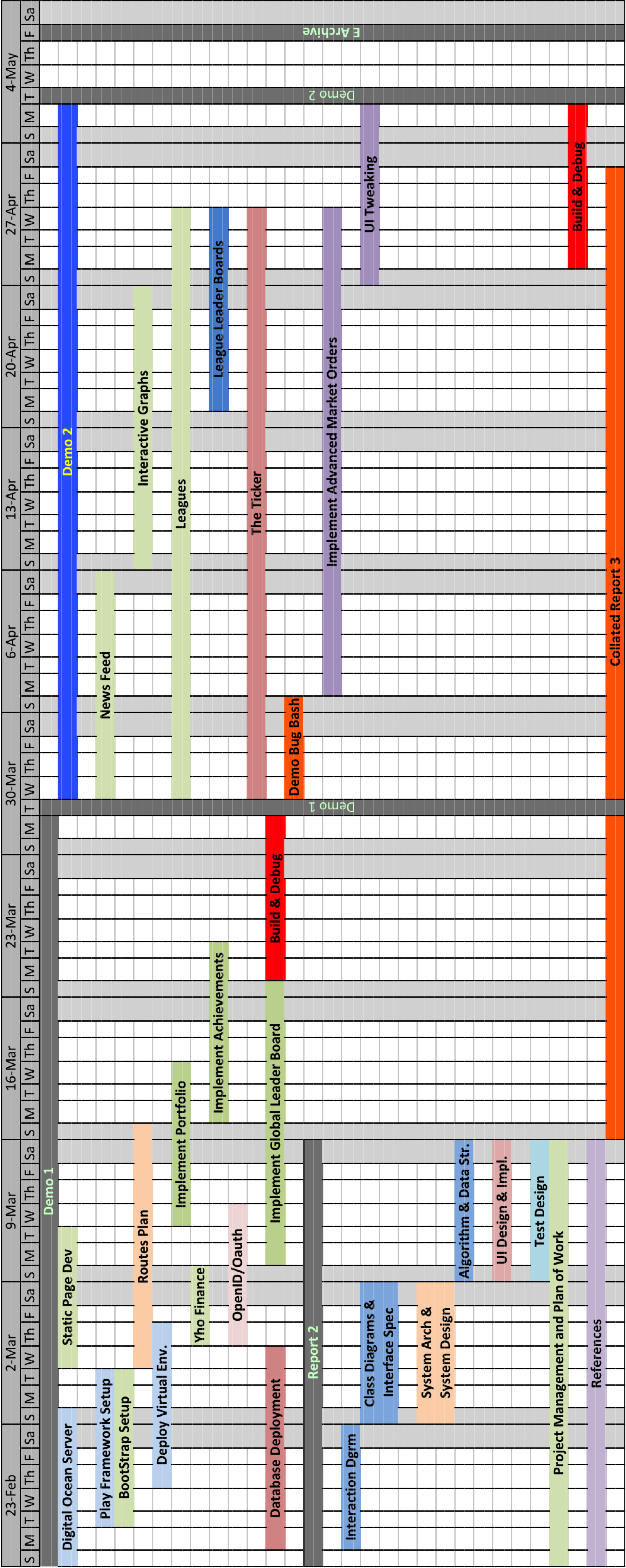
\includegraphics[height=9in]{./img/planOfWork.png}
\caption{This chart is the roadmap to meeting all our milestones.}
\end{figure}

%\eject \pdfpagewidth=8.5in \pdfpageheight=11in

% Chapter 7
% This includes timelines, how the team divided up work, etc..
% Include Contributions page
\chapter{Project Management}
\label{managment}
%\section{Coordination and Division of Labor}
%\section{User Story Matrix}
\section{Report 1 Contributions}

\begin{centering} % Aligns center
\renewcommand\arraystretch{2} % Causes rows to be spaced slightly more
\begin{tabular}{cc|c|c|c|c|c|c|} % Creates a table with centered
                                 % columns "c", separated by bars "|"
\cline{3-8} % draw a horizontal line across columsn 3-8
& & \multicolumn{6}{ c| }{Names} \\ \cline{1-8}
\multicolumn{1}{|c|}{Category} & \multicolumn{1}{c|}{Points} &
David P & David K & Jesse Z & Evan A & Eric J & Chris M \\ \cline{1-8}
\multicolumn{1}{|c|}{Project Management} & \multicolumn{1}{c|}{10 Points} &
100\% & 0\% & 0\% & 0\% & 0\% & 0\% \\ \cline{1-8}
\multicolumn{1}{|c|}{Customer Requirements} & \multicolumn{1}{c|}{9 Points} &
50\% & 0\% & 0\% & 0\% & 0\% & 50\% \\ \cline{1-8}
\multicolumn{1}{|c|}{System Requirements} & \multicolumn{1}{c|}{6 Points} &
20\% & 20\% & 0\% & 0\% & 30\% & 30\% \\ \cline{1-8}
\multicolumn{1}{|c|}{Functional Requirements} & \multicolumn{1}{c|}{30 Points} &
0\% & 0\% & 0\% & 33\% & 33\% & 33\% \\ \cline{1-8}
\multicolumn{1}{|c|}{User Interface Specifications} & \multicolumn{1}{c|}{15 Points} &
50\% & 50\% & 0\% & 0\% & 0\% & 0\% \\ \cline{1-8}
\multicolumn{1}{|c|}{Domain Analysis} & \multicolumn{1}{c|}{25 Points} &
0\% & 0\% & 80\% & 0\% & 20\% & 0\% \\ \cline{1-8}
\multicolumn{1}{|c|}{Plan of Work} & \multicolumn{1}{c|}{5 Points} &
100\% & 0\% & 0\% & 0\% & 0\% & 0\% \\ \cline{1-8}
\end{tabular}
\end{centering}


% References
\bibliography{citations}


\end{document}
